\problemname{Happy Hookup}

% optionally define variables/limits for this problem
\newcommand{\maxn}{10^5}

It has happened! You found a match!
Excitedly, your match Hannah and you have decided to have a morning stroll together.
Since the two of you live in different cities, you decide to meetup at a train station.

Getting to your respective cities' train station is no problem.
However, the ongoing renovations of the national train network heavily impact the available connections.
Some of them are not available at all, and some others are only one-way.
This makes it uncertain whether you can meet up at all.

\begin{figure}[h]
	\centering
	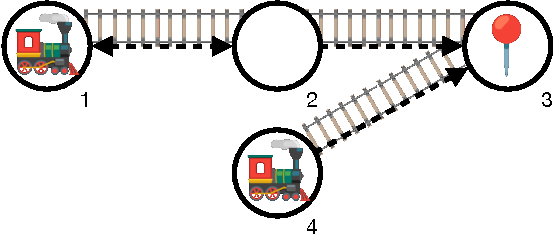
\includegraphics[width=.5\textwidth]{sample_hookup}
	\caption{Visualization of the third sample.
		Hannah starts from station $4$, and you start from station $1$.
		You can both reach station $3$ for your meet-up.
	}
\end{figure}


You have found a list of the available train connections online.
A train station is suitable for your meet-up if both Hannah and you can reach it.
Determine whether there is a suitable train station or whether it is necessary to move the morning stroll to another day.

\begin{Input}
    The input consists of:
	\begin{itemize}
		\item One line with two integers $n$ and $m$ ($2 \leq n \leq \maxn$, $0 \leq m \leq \maxn$), the number of train stations and train connections, respectively.
		\item $m$ lines, each with two integers $x$ and $y$ ($1 \leq x, y \leq n$, $x \neq y$), denoting a direct train connection from train station $x$ to train station $y$.
		\item One line with two integers $a$ and $b$ ($1 \leq a,b \leq n$, $a \neq b$), the train stations you and Hannah start from, respectively.
	\end{itemize}
	It is guaranteed that no train connection is listed multiple times.
\end{Input}

\begin{Output}
	If no suitable train station exists, output ``\texttt{no}''.

	Otherwise, output ``\texttt{yes}'', followed by the train station.
	If there are multiple valid solutions, you may output any one of them.
\end{Output}
